\documentclass{jsarticle}
\usepackage[dvipdfmx]{graphicx}
\usepackage{listings,jlisting}
\usepackage{float}

\title{情報工学実験1数理計画法}

\author{学生番号4617043 神保光洋}
\date{\today}
\begin{document}
\maketitle

\section{実験の要旨}
c言語において乱数を発生させる際に使うrand()関数を用いたものとMersenne Twister(MT)を
を使いディジタル通信システムと謝り訂正符号の理解を深める。

\section{実験の目的}
通信システムの「シュミレーション」を通し、ディジタル通信システムと誤り訂正符号の
理解を深める。

\section{実験の原理}
\subsection{誤り訂正符号}
情報を伝えるとき、できるだけ正確に伝えるための仕組みであり、
送信メッセージに助長性を持たせることで通信路で発生した
誤りを訂正することが可能である。

\subsection(2元対称通信路(BSC))
2元記号$\{ 0, 1 \} $が誤り率 $\varepsilon (0 \leq \varepsilon \leq 1)$ で"0"が"1"に
誤り、"1"が"0"に誤る。


\section{実験の装置あるいは実験手順}
確率モデルで表現される通信路(2元対称通信路)
を、乱数を用いて実装rand()関数、Mersenne Twister(MT)の2種類の擬似乱数生成器を用いる。

\subsection{情報系列$w = (w_1, w_2, ...,w_k)$の生成}
0以上1以下の乱数を発生させ、乱数が0.5以下ならば"0"、0.5 < 乱数ならば
"1"とし情報系列$w$を生成(ここの0.5はどうでもよく自分は$\varepsilon$を用いた)。

\subsection{BSCでん雑音$e = (e_1, e_2, ..., e_k)$の発生と受信系列$y = (y_1, y_2, ...,y_k)の生成$}
\subsubsection{BSCでの雑音$e= (e_1, e_2, ..., e_k)$の発生}
0以上1以下の乱数を発生させ、乱数が$\varepsilon$以下ならば"1"(誤りあり)、$\varepsilon$ < 乱数ならば
"1"(誤りなし)とし雑音系列$e$を生成


\subsubsection{受信系列$y = (y_1, y_2, ..., y_k))$ の生成}
情報系列$w$と雑音系列$e$の各要素の排他的論理和

$$
y_i - w_i \oplus e_i, i \in \{ 1,2,...,k \}
$$

を計算
\subsection{誤りビット数の算出}
情報系列$w$と受信系列$y$の情報ビット$w_i$と受信ビット$y_i$が異なる
数を数える。

\subsection{ビット誤り率$P_e$の計算}
1~3を十分な精度が得られるまで繰り返し、ビット誤り率$P_e$を求める。
$P_e$は誤ったビットの総数を送信したビットの総数で割ったものである。
\subsection{1~4を各 $\varepsilon$について実行する}


\section{結果}
結果は以下のようになった。

\begin{table}[htb]
  \begin{center}
    \caption{$\varepsilon$と$P_{dec}$の関係}
    \begin{tabular}{|c|c|c|} \hline
      $\varepsilon$ & rand()の$P_{dec}$ & $MT$の$P_{dec}$ \\ \hline
      0.000010 & 0.000000   &  0.000011 \\ \hline
      0.000020 & 0.000020   &  0.000021 \\ \hline
      0.000030 & 0.000028   &  0.000032 \\ \hline
      0.000040 & 0.000035   &  0.000041 \\ \hline
      0.000050 & 0.000050   &  0.000048 \\ \hline
      0.000060 & 0.000068   &  0.000052 \\ \hline
      0.000070 & 0.000045   &  0.000069 \\ \hline
      0.000080 & 0.000090   &  0.000080 \\ \hline
      0.000090 & 0.000085   &  0.000091 \\ \hline
      0.000100 & 0.000115   &  0.000104 \\ \hline
    \end{tabular}
  \end{center}
\end{table}

\begin{figure}[H]
  \centering
  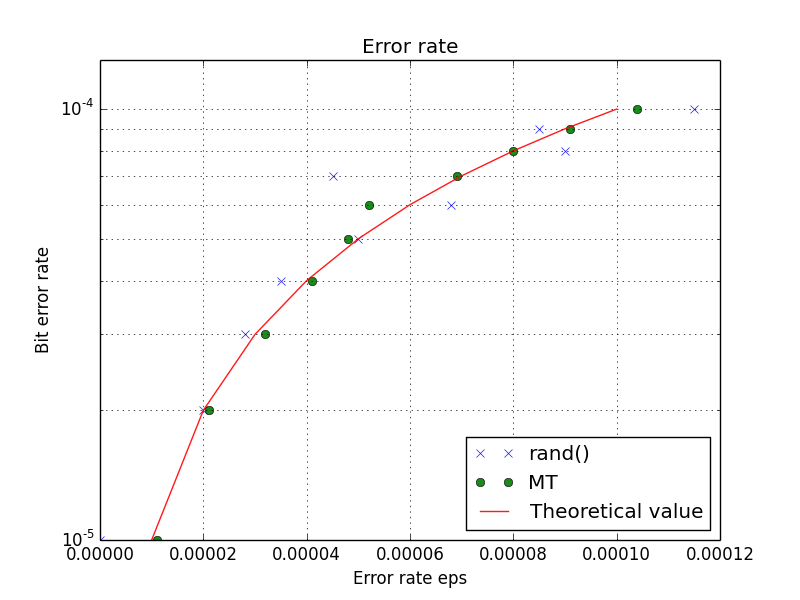
\includegraphics[width=12cm]{./graph1.png}
  \caption{最急降下法が生成した二次元配列}
\end{figure}

\section{検討・考察}

\section{検討事項}
\subsection{シュミレーションによるBERと理論値がほぼ同じ値になるにはどの程度のシュミレーション回数を実行する必要があるか}
1何度か試行した結果100万回以上必要であることがわかる。

\subsection{$\varepsilon$を非常に小さくした場合、検討事項1-1はどうなるか。}
上ののグラフより誤り率が小さいほど理論値に近づいていることが見て取れるため
試行回数は100万回よりも少なくて良いと考察される。


\subsection{rand()とMTの違いは何か、検討事項1-1と1-2を絡めて考察せよ}
MTはrand()よりも周期が大きいため回数を重ねるとrand()よりもMTの方が
より正確な乱数を生成する。このことより検定事項1-1ではシュミレーション回数
を大きくしていった際よりMTの方が理論値に近くと考察される。

\section{結論}
rand()はMTに比べ沢山の乱数を生成することに向いていないが
コンピュータの記憶容量の消費はMTに比べ小さく少量の
乱数生成に向いていると結論付けられる。

\section{参考文献}
\begin{thebibliography}{9}
  \bibitem{key1} やさしいC(第5版)・高橋麻奈
\end{thebibliography}

\section{付録}
実験で使用したプログラムは以下のようになる。
\lstinputlisting[caption = rand().c ,label = program1]{./rand.c}
\lstinputlisting[caption = MT.c ,label = program2]{./MT.cpp}

\end{document}
